\documentclass{beamer}
\usetheme{KUL}
\usepackage{multirow}
\usepackage{multicol}
\usepackage{tikz}
\usepackage{ulem}
\usepackage{siunitx}
\newcommand
\itemS{
\item[\textbf{\S}]}
\definecolor{darkgreen}{rgb}{0,0.598,0.199}
\usepackage{times} % set font on times new roman
\usepackage{eurosym} % package for Euro sign
\usepackage{lineno}   % package for line numbering
\usepackage{subcaption}  % this package enables one to put several
% figures next to each other
\usepackage{textcomp}
\usepackage{setspace}
\usepackage{gensymb}
\usepackage{url}
\usepackage[backend=biber,style=numeric-comp,sorting=none]{biblatex}
\addbibresource{bib.bib}
\usepackage{hyperref} % this is for url links

%----------------------------------
% Fill in the essential Information
%----------------------------------

\title[Candlestick Patterns]{Performance of candlestick patterns on
intraday market data}
\subtitle{Seminar}
\author[W.\ Notermans]{Wout Notermans} % between [] is short name,
% between {} is long name
\date{May 14, 2025} % Here you can also just type something, e.g.
% October 10, 2017
\institute[KU Leuven]{Faculty of Science\\ Department of
Mathematics\\ Section of Statistics and Risk}

%----------------------------------
% ACTUAL PRESENTATION STARTS HERE
%----------------------------------

\begin{document}

% TITLE PAGE
{
  \setbeamertemplate{headline}{} %define local, empty header for title page
  \setbeamertemplate{footline}{} %define local, empty footer for title page
  \maketitle
}
\addtocounter{framenumber}{-1} % We don't count the title page

% \begin{kulblock}{Landslide}
%     A landslide is the downhill movement of soil mass
% \end{kulblock}

% ------------
% Introduction
% ------------

\section{Introduction}

\begin{frame}{Table of contents}
  \tableofcontents
\end{frame}

\begin{frame}[noframenumbering]{Table of contents}
  \tableofcontents[currentsection]
\end{frame}

\begin{frame}{Stock price \cite{berkshirehathaway}}
  \centering
  \includegraphics[width=0.8\textwidth]{Images/BRK.A_line.pdf}\\

\end{frame}

\begin{frame}[noframenumbering]{Stock price \cite{berkshirehathaway}}
  \centering
  \includegraphics[width=0.8\textwidth]{Images/BRK.A_candle.pdf}
\end{frame}

\begin{frame}{Candlestick construction}
  \centering
  \includegraphics[width=\textwidth]{Images/candlestick_construction.png}
  Construction of a candlestick \cite{chen2020}.
\end{frame}

\begin{frame}{Candlestick pattern examples}
  \centering
  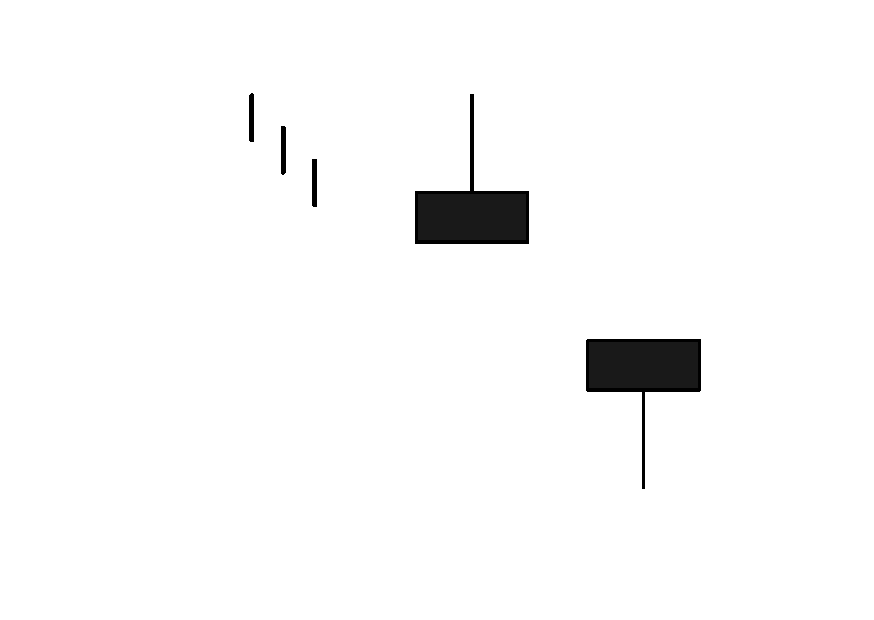
\includegraphics[width=0.5\textwidth]{Images/window_falling.pdf}%
  \includegraphics[width=0.5\textwidth]{Images/meeting_lines_bearish.pdf}
\end{frame}

\begin{frame}{History}
  \begin{itemize}
    \item Developed in the 1700s in Japan.
    \item Remained exclusive to the East until 1991.
    \item This is reflected in the literature.
    \item Quite well-known technical analysis technique.
  \end{itemize}
\end{frame}

\begin{frame}{Literature}
  \begin{itemize}
    \item Literature split between machine learning and rule based approach.
    \item Results are very split.
    \item Very few publications about intraday market data.
  \end{itemize}
\end{frame}

\begin{frame}
  \begin{kulblock}{Research question}
    Do candlestick patterns possess any predictive power on intraday market data?
  \end{kulblock}
\end{frame}

% -----------
% Methodology
% -----------

\section{Methodology}

\begin{frame}[noframenumbering]{Table of contents}
  \tableofcontents[currentsection]
\end{frame}

\begin{frame}{Overview}
  \begin{itemize}
    \item Selection of data sets.
    \item Preprocessing of the data.
    \item Trends and technical indicators.
    \item Pattern detection.
    \item Pattern evaluation.
  \end{itemize}
\end{frame}

\begin{frame}{Data sets}
  \begin{itemize}
    \item BND: Bonds.
    \item GLD: Gold.
    \item QQQ: Stocks.
    \item SPY: Stocks.
    \item Wiener: Generated.
  \end{itemize}
\end{frame}

\begin{frame}{Preprocessing}
  \begin{itemize}
    \item Filter pre/after-market and economic news.
    \item Missing data $\rightarrow$ interpolation.
    \item Aggregation.
    \item Splitting of the data set for calibration.
  \end{itemize}
\end{frame}

\begin{frame}{Preprocessing: calibration}
  \scalebox{0.8}{
    \begin{tabular}{cccccc}
      \hline
      & Doji & Short & Normal & Tall & Extremely tall \\
      Real body & $[0-10)$ & $[10-30)$ & $[30-70)$ & $[70-100]$ &  \\ \hline
      Shadow & $[0-10)$ & $[10-30)$ & $[30-70)$ & $[70-90)$ & $[90-100]$ \\ \hline
    \end{tabular}
  }
  \centering\\[1em]
  Percentiles of real bodies and shadows \cite{etschberger2006}.\\
  \includegraphics[width=0.5\textwidth]{Images/matching_low.pdf}
\end{frame}

\begin{frame}{Preprocessing: calibration}
  \begin{itemize}
    \item Assumes length and color candle independent.
    \item Has to be checked $\rightarrow$ Kolmogorov-Smirnov test.
      $$H_0: W = B \qquad H_1: W \neq B.$$
    \item Reject at 5\% significance.
  \end{itemize}
\end{frame}

\begin{frame}{Trend}
  \begin{itemize}
    \item Many patterns are only valid when the correct trend is present.
    \item Multiple ways of defining the trend in the literature.
    \item Example: count in/decreases in the moving average.
  \end{itemize}
\end{frame}

\begin{frame}{Technical indicators}
  \begin{itemize}
    \item Values calculated from asset prices and volume.
    \item Some publications only find significant patterns when combining them with technical indicators.
    \item Quite a number found in the literature.
    \item Example: triple exponential (TRIX).
  \end{itemize}
\end{frame}

\begin{frame}{Pattern detection}
  \begin{itemize}
    \item Patterns are vaguely defined at best: a rigid classification is necessary.
    \item The paper ``A formal approach to candlestick pattern classification in financial time series'' does exactly this \cite{hu2019}.
    \item Define 103 candlestick patterns with strict conditions.
  \end{itemize}
\end{frame}

\begin{frame}{Pattern detection: example}
  \centering
  \includegraphics[width=0.75\textwidth]{Images/doji_star_bearish.pdf}
\end{frame}

\begin{frame}{Pattern detection: prediction}
  \begin{itemize}
    \item Typically classified as buy/sell signal.
    \item Look at the results themselves instead of the predictions.
  \end{itemize}
  \centering
  \includegraphics[width=0.6\textwidth]{Images/stick_sandwich.pdf}
\end{frame}

\begin{frame}{Pattern evaluation}
  \begin{itemize}
    \item Buy/sell after pattern is detected.
    \item Make use of stop loss/take profit margins.
    \item This gives us a winning rate.
    \item Test significance with binomial test. \\ $$H_0:\pi=0.5\qquad\qquad H_1:\pi>0.5$$
  \end{itemize}
\end{frame}

\begin{frame}{Pattern evaluation: stop loss/take profit \cite{berkshirehathaway}}
  \centering
  \includegraphics[width=0.75\textwidth]{Images/BRK.A_candle_stop_loss.pdf}
\end{frame}

\begin{frame}{Pattern evaluation: profitability score}
  Quantify profitability score with three factors:
  \begin{enumerate}
    \item The number of detected patterns.
      $$\max\left(\dfrac{200}{1+\exp\left(-\dfrac{n-100}{100}\right)}-100,0\right)$$
    \item The win rate (deviation from 50\%).
    \item The significance.
  \end{enumerate}
\end{frame}

% -------
% Results
% -------

\section{Results}

\begin{frame}[noframenumbering]{Table of contents}
  \tableofcontents[currentsection]
\end{frame}

\begin{frame}{Detection results}
  \begin{itemize}
    \item Not many ``gapping" patterns.
    \item Some patterns are rare due to stringent conditions.
  \end{itemize}
  \centering
  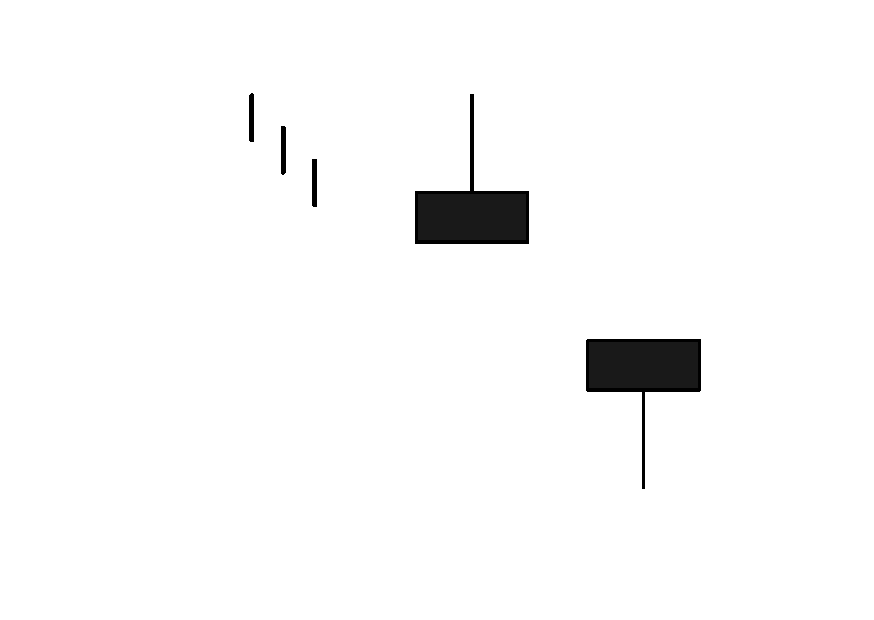
\includegraphics[width=0.5\textwidth]{Images/window_falling.pdf}%
  \includegraphics[width=0.5\textwidth]{Images/evening_doji_star.pdf}
\end{frame}

\begin{frame}{Evaluation results: significance}
  \begin{itemize}
    \item Significant patterns are found.
    \item Many more significant buy than sell signals.
    \item A lot of variance between data sets/asset types.
    \item Aggregation decreases significance but not profitability.
  \end{itemize}
\end{frame}

\begin{frame}{Evaluation results: effect of data set}
  \centering
  \includegraphics[width=0.8\textwidth]{Images/mean_profit_diff_data.pdf}
\end{frame}

\begin{frame}{Evaluation results: effect of time interval}
  \centering
  \includegraphics[width=0.8\textwidth]{Images/mean_profit_diff_minutes.pdf}
\end{frame}

\begin{frame}{Evaluation results: effect of news}
  \centering
  \includegraphics[width=0.8\textwidth]{Images/mean_profit_news.pdf}
\end{frame}

\begin{frame}{Evaluation results: no effect}
  \begin{itemize}
    \item Different start and end times.
    \item Filtering based on technical indicators.
    \item Averaging methods: SMA, WMA, EMA.
    \item Trend defining methods.
  \end{itemize}
\end{frame}

\begin{frame}{Evaluation results: MVP}
  \centering
  \includegraphics[width=0.75\textwidth]{Images/stick_sandwich.pdf}
\end{frame}

% ----------
% Conclusion
% ----------

\section{Conclusion and further research}

\begin{frame}[noframenumbering]{Table of contents}
  \tableofcontents[currentsection]
\end{frame}

\begin{frame}
  \begin{kulblock}{Research question}
    Do candlestick patterns possess any predictive power on intraday market data?
  \end{kulblock}
\end{frame}

\begin{frame}{Conclusion}
  \begin{itemize}
    \item Some patterns do appear to possess (consistent) significant predictive power.
    \item This mainly holds true for buy signals.
    \item There is a lot of variance to these results.
  \end{itemize}
\end{frame}

\begin{frame}{Further research}
  \begin{itemize}
    \item Machine learning-based approach to detection.
    \item Fuzzy rules for detection.
    \item ``Evolving margins'' evaluation.
  \end{itemize}
\end{frame}

% ------------
% Bibliography
% ------------

\section*{Bibliography}

\begin{frame}[noframenumbering,allowframebreaks]
  \printbibliography
\end{frame}

\section*{}

\begin{frame}
  \begin{center}
    \color{cyan} \LARGE Questions?
  \end{center}
\end{frame}

\end{document}
